\section{Część realizująca sterowanie bezpośrednie (,,niższego poziomu'')}
\label{sec:czesc-nizsza}

%TODO: napisać ten podrozdział
%-------------------------------------------------
\subsection{Pakiet Simulink jako narzędzie realizujące sterowanie}
\label{sub:czesc-nizsza-matlab}

\cite{Trawinski2011}

%TODO: wrzucić i opisać rysunek modelu

\begin{figure}
    \centering
    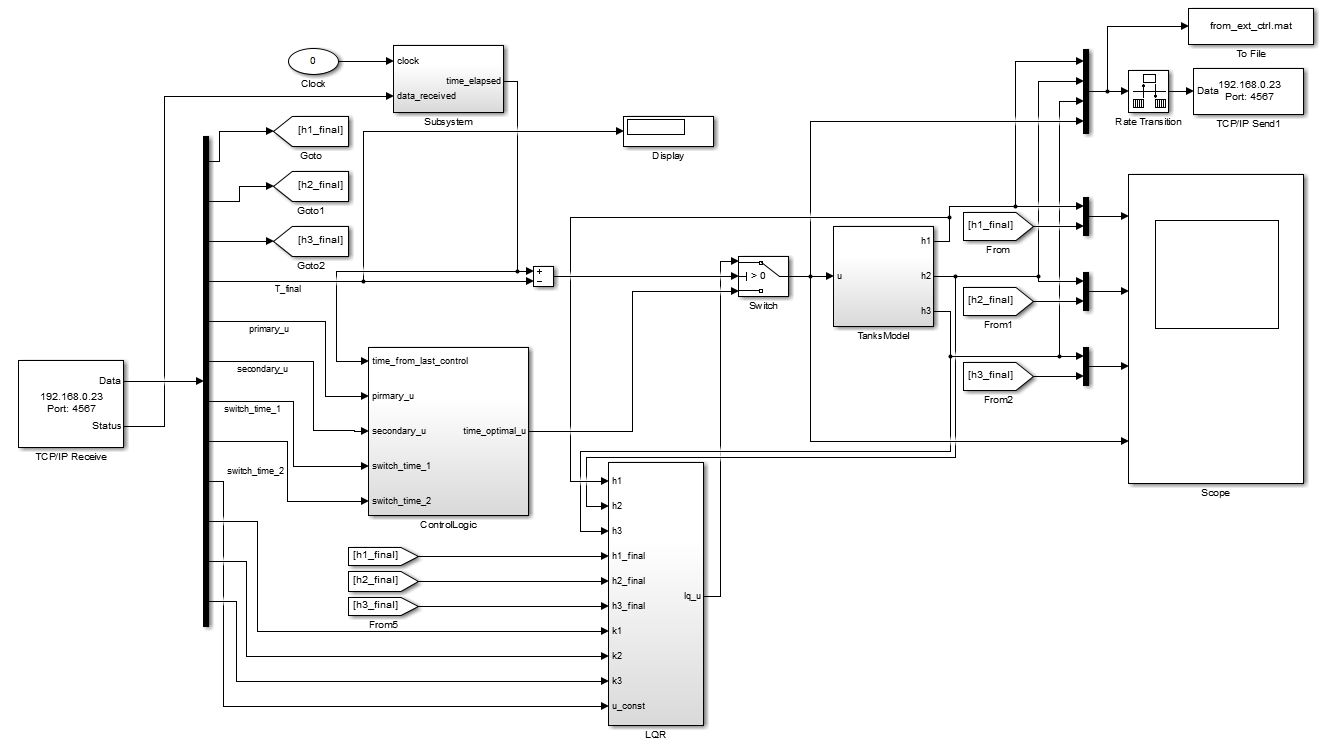
\includegraphics[scale=0.65,angle=90]{Grafika/simulink_model}
    \caption{Model niższego poziomu aplikacji w programie Simulink. Źródło: własne.}
    \label{fig:simulinkmodel}
\end{figure}

